\section{S-turn}
%
The third developed example is a simple S-shaped turn also known as chicane manoeuvre. In the specific this sample track is composed by four sections. The first is a straight line of $200\,\si{\metre}$, followed by a clockwise (left) turn of $90\,\si{\degree}$ with radius of curvature equal to $50\,\si{\metre}$ and a subsequent equal but in the counter clockwise direction. Finally at the exit of the chicane there is a straight line equal to the first one ($200\,\si{\metre}$). The road is $12\,\si{\metre}$ wide as usual for race circuit.\\
This example is, again, particularly interesting test bench for the model and the optimal control set-up. The chicane is a typical section which is present in most of the real circuit, an example above all is the Mugello circuit.\\
The problem that the author aim to solve is similar to the U-turn manoeuvre, travel the chicane at the peak performance of the motorcycle.
%
\subsection{Solution approach}
%
This problem cannot be solved in a straight forward fashion as in the U-turn example. It it complex and not converging without the right guess of state controls and lagrange multipliers.\\
The solution can be obtained using homotopy. The first solution is found imposing the well known steady state in the mayer term and as initial condition. The final conditions are left free. The following step is imposing the equality of initial and final condition. Then the initial condition are liberated from the constraint in the mayer term. At the last step the tolerances of the penalties are pushed to reach the maximum performance.
%
\subsection{Results and comparison}
%
The results obtained are somehow similar to the U-shaped turn. this behaviour was expected since the two manoeuvres are derived following the same approach.\\
%
\begin{figure}[!htb]
    \centering
    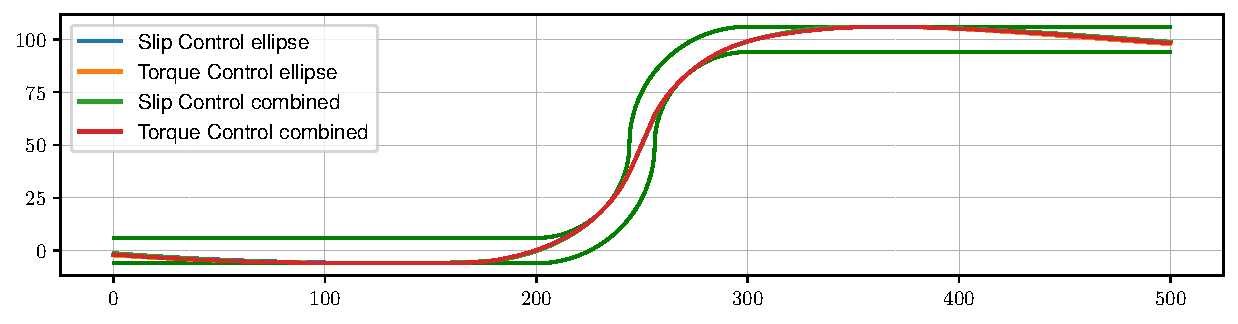
\includegraphics[width=\linewidth]{S-turn/Track_S_confront.pdf}
    \caption{Trajectory in S-turn}
    \label{fig:STrajectory}
\end{figure}
%
The trajectories obtained in the four models are really close to each others. This can be seen from figure \ref{fig:STrajectory} and in figure \ref{fig:S2b}. The motorcycle reach the external border, lean inside, then counter steer and exit touching the outside border.\\
A close look to figure \ref{fig:S2b} reveal that the four model follow exactly the same trajectory when in turning manoeuvre.
%
\begin{figure}[!htb]
    \begin{subfigure}{0.5\linewidth}
        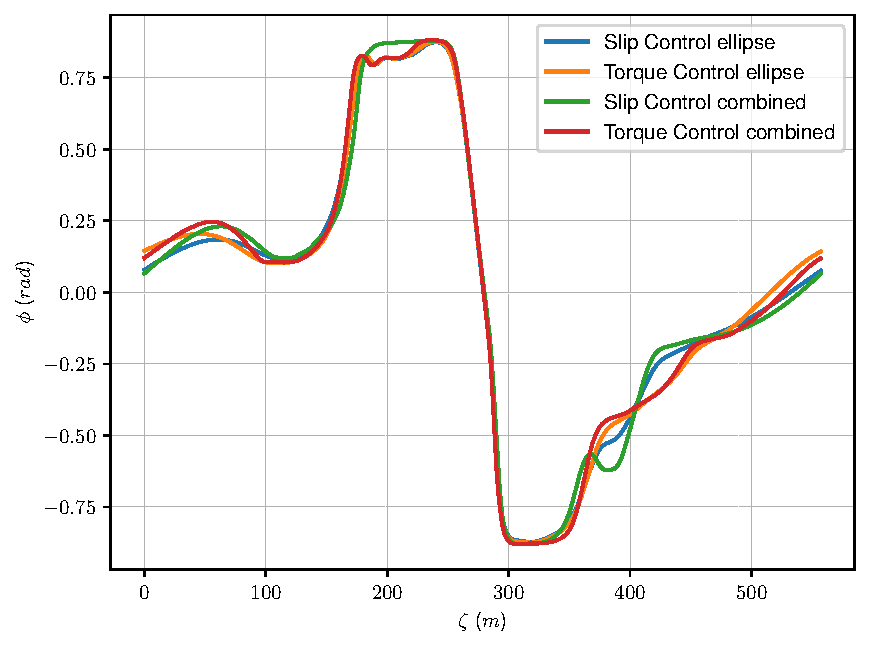
\includegraphics[width=\linewidth]{S-turn/phi_S_confront.pdf}
        \caption{Roll angle}
        \label{fig:S2a}
    \end{subfigure}%
    \begin{subfigure}{0.5\linewidth}
        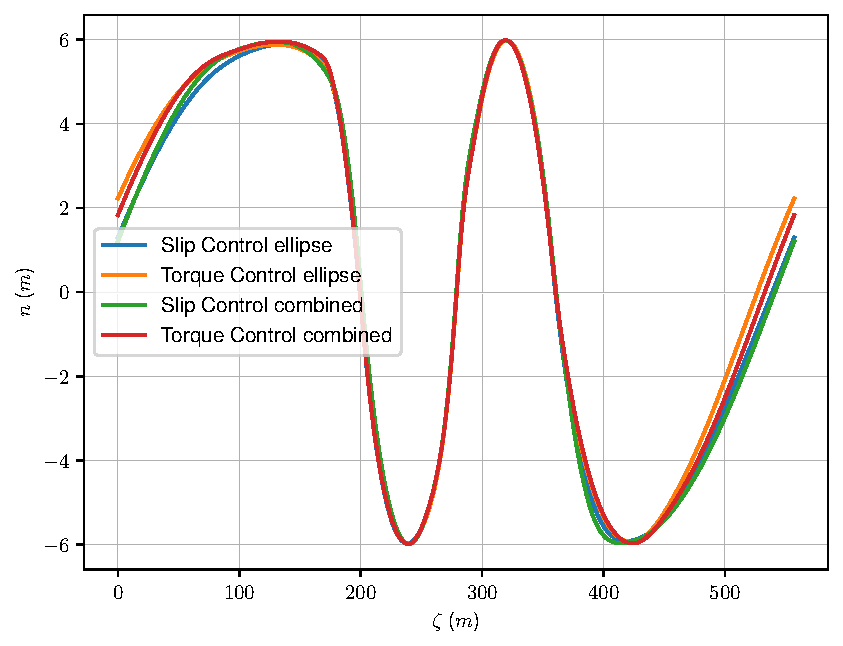
\includegraphics[width=\linewidth]{S-turn/n_S_confront.pdf}
        \caption{Centreline deviation}
        \label{fig:S2b}
    \end{subfigure}
    \caption{Confront of roll angle and centreline deviation in S-turn}
\end{figure}
%
%
\begin{figure}[!htb]
    \begin{subfigure}{0.5\linewidth}
        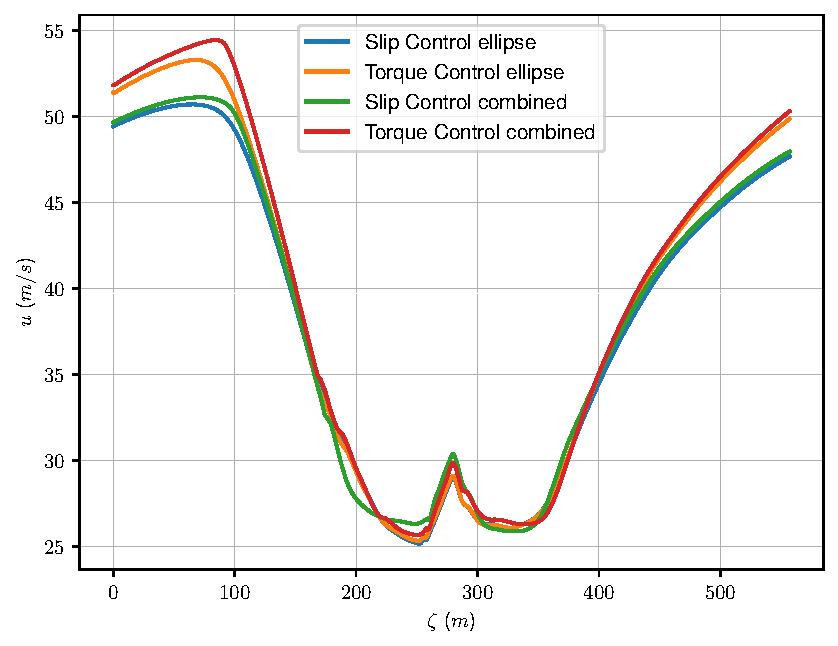
\includegraphics[width=\linewidth]{S-turn/u_S_confront.pdf}
        \caption{Longitudinal velocity}
        \label{fig:S1a}
    \end{subfigure}%
    \begin{subfigure}{0.5\linewidth}
        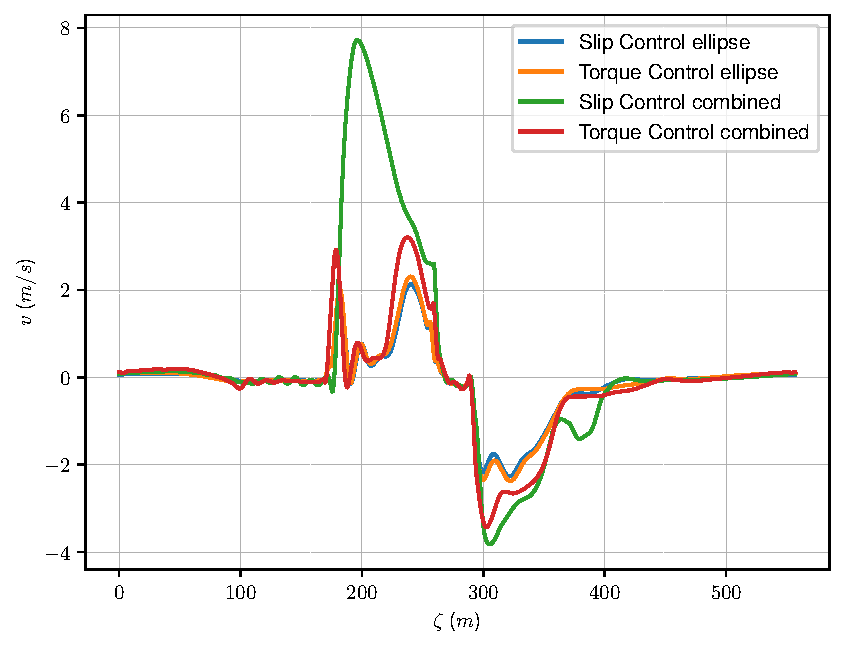
\includegraphics[width=\linewidth]{S-turn/v_S_confront.pdf}
        \caption{Lateral velocity}
        \label{fig:S1b}
    \end{subfigure}
    \caption{Confront of velocity in S-turn}
\end{figure}
%
%
\begin{figure}[!htb]
    \begin{subfigure}{0.5\linewidth}
        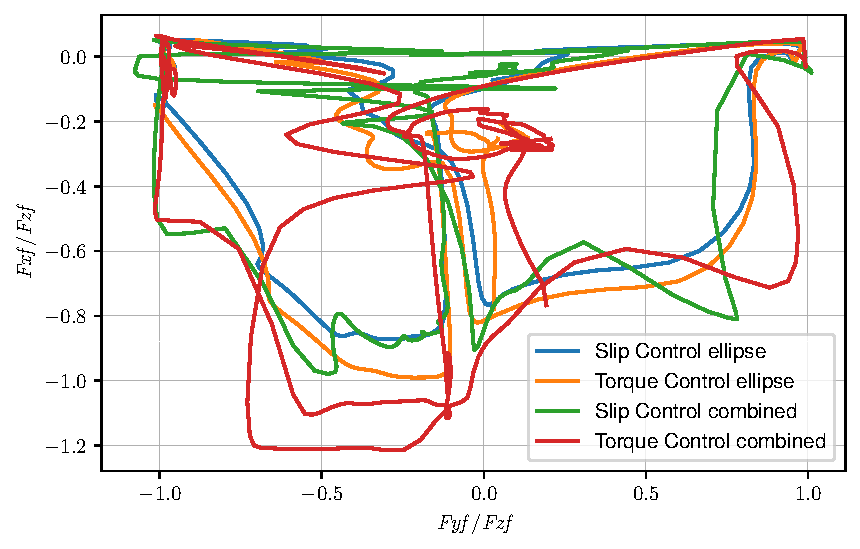
\includegraphics[width=\linewidth]{S-turn/EFront_S_confront.pdf}
        \caption{Front}
        \label{fig:SEa}
    \end{subfigure}%
    \begin{subfigure}{0.5\linewidth}
        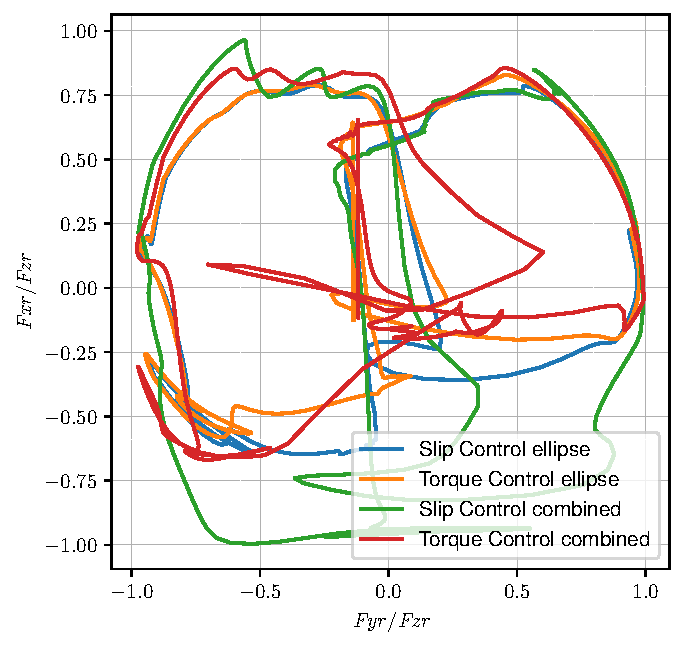
\includegraphics[width=\linewidth]{S-turn/ERear_S_confront.pdf}
        \caption{Rear}
        \label{fig:SEb}
    \end{subfigure}
    \caption{Ellipse of adherence S-turn}
\end{figure}
%
\\
%
The velocity profiles are reported in figure \ref{fig:S1a} and \ref{fig:S1b}. It shows again a much aggressive manoeuvre for the torque control models. However, the lateral velocity peak can be found for the slip control in combined model.\\
The other performance indexes are the adherence ellipses of front and rear tyre. In this case we can see in figure \ref{fig:SEa} and \ref{fig:SEb}. In acceleration and turning all four models reach almost the same performances.\\
In braking condition instead the torque controlled model shows a different behaviour. In fact, those exploit much more the front wheel. This is caused by the vertical load distribution.\\ 
As highlighted in figure \ref{fig:SFZF} and \ref{fig:SFZR} during the braking phase left the rear axle unloaded. Moreover the figure \ref{fig:SEa} and \ref{fig:SEb} are the normalized forces with the vertical load. However, longitudinal and lateral forces are not linear function of the load. For this reason one should scale the forces by a term that is considering this factor. For instance the peak value of the forces (parameter $D$ of the magic formula\cite{pacejka2012tire}.)  
%
\begin{figure}[!htb]
    \begin{subfigure}{0.5\linewidth}
        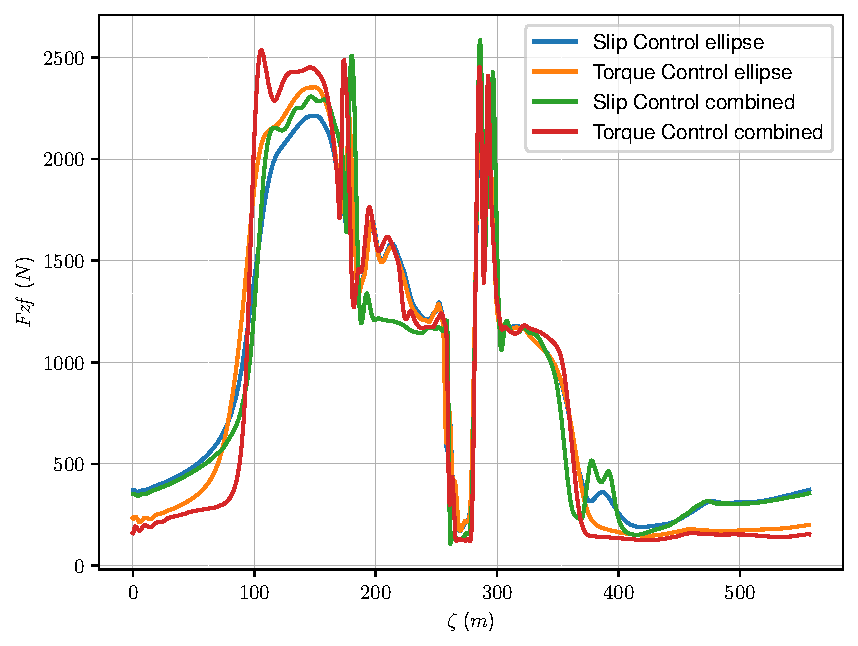
\includegraphics[width=\linewidth]{S-turn/Fzf_S_confront.pdf}
        \caption{Front}
        \label{fig:SFZF}
    \end{subfigure}%
    \begin{subfigure}{0.5\linewidth}
        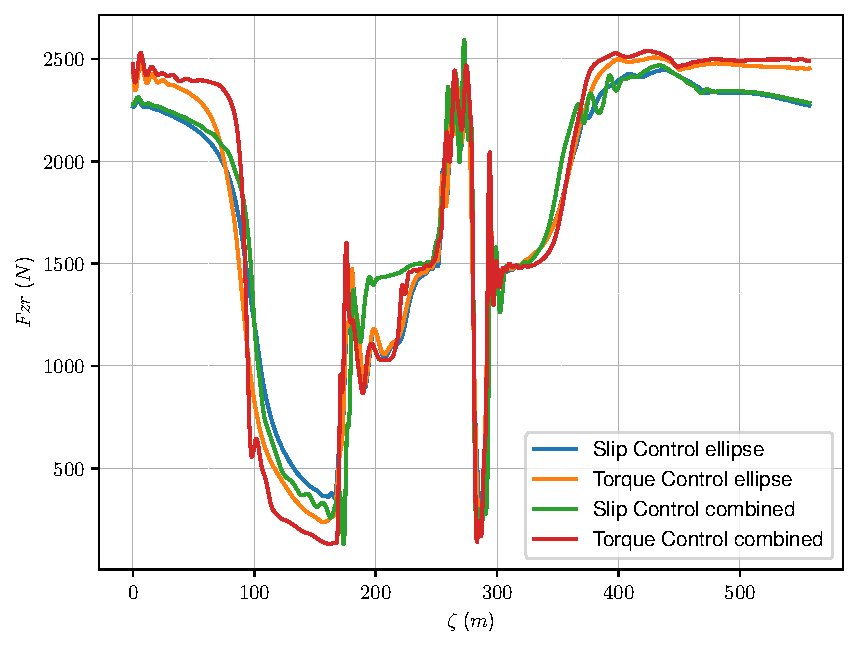
\includegraphics[width=\linewidth]{S-turn/Fzr_S_confront.pdf}
        \caption{Rear}
        \label{fig:SFZR}
    \end{subfigure}
    \caption{Vertical forces in S-turn}
\end{figure}
%